\documentclass[11pt]{article}
\usepackage{report}
\newlength\figureheight 
\newlength\figurewidth
\newif\iftikz
\tikztrue


\begin{document}
\section{Checking data for heat capacity}
In figure \ref{heatCap} we can see how the two theories used to calculate the heat capacities seem to yeild similair results. This is a good indication that the simulation software is correctly implemented.
\begin{figure}[H]
	\centering
	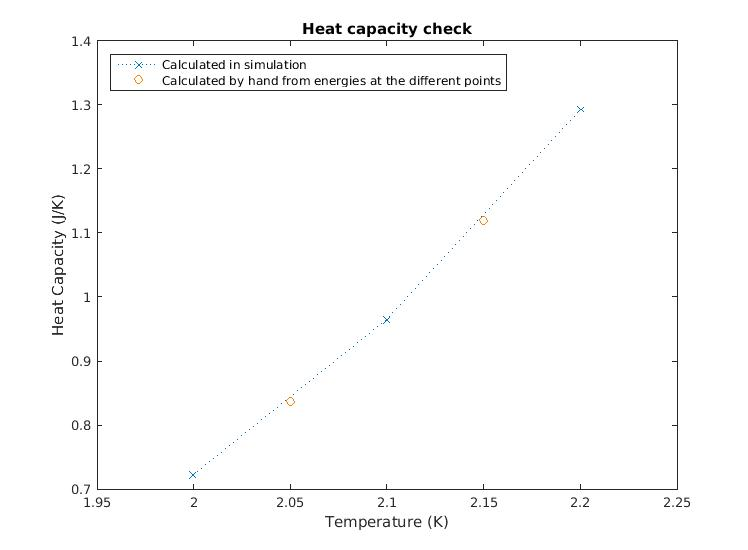
\includegraphics[width=1\textwidth]{../../plots/heatCap}
	\caption{Looking at the heat capacities at different temperatures for different systemsizes}
	\label{fig:heatCap}
\end{figure}

\section{Phase Transition and Size Dependency}
In figure \ref{fig:phaseTrans} and \ref{fig:mag} we can see the transition for the system from beeing magnetic and ordered not non-magnetic or unordered. We can see there is behavior closer to the analytical one when the system is bigger and the simulation seem to go further and further away from it when the system is smaller, both for the magnetic transition and the heat capacity peaks that occour around the curie temperature.

\begin{figure}[H]
	\centering
	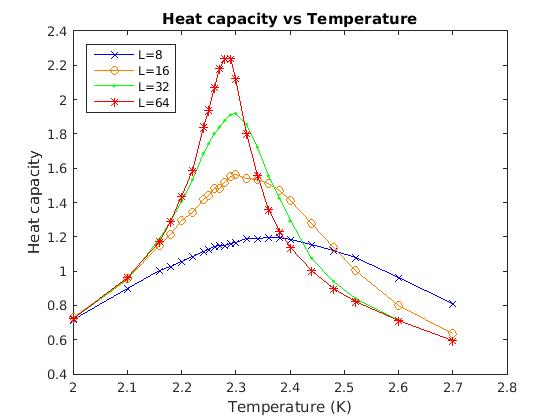
\includegraphics[width=1\textwidth]{../../plots/phaseTrans}
	\caption{Looking the magnetic phase transition for the system at different sizes}
	\label{fig:phaseTrans}
\end{figure}

\begin{figure}[H]
	\centering
	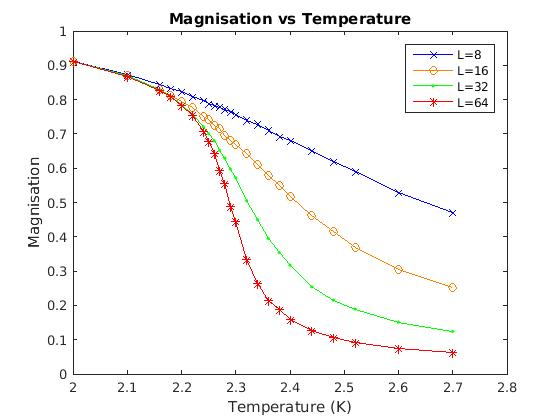
\includegraphics[width=1\textwidth]{../../plots/mag}
	\caption{Picture looking at different way calculated heat capacities}
	\label{fig:mag}
\end{figure}

\section{Cluster Update}
The plot of the magnitisation for different system sizes is depicted in figure \ref{fig:clusterPlot}. The linear fit of the data yeilded a a value on $\beta$ to be $0.125046$. As we can see the (atleast if we compare the smallest system with the biggest one) system more clearly resembles the analytical theory with a bigger system. Thus we can see the dependency of system size for the wolf cluster method.

\begin{figure}[H]
	\centering
	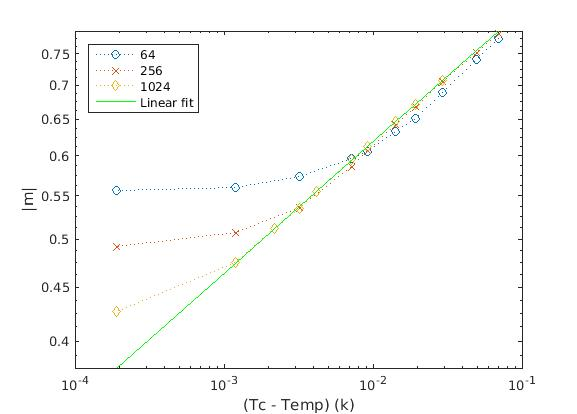
\includegraphics[width=1\textwidth]{../../plots/clusterPlot}
	\caption{Here we can see the magnitude of the magnisation in the system plotted against the temperature around $T_c$}
	\label{fig:clusterPlot}
\end{figure}

\section{Time Correlation}

\begin{figure}[H]
	\centering
	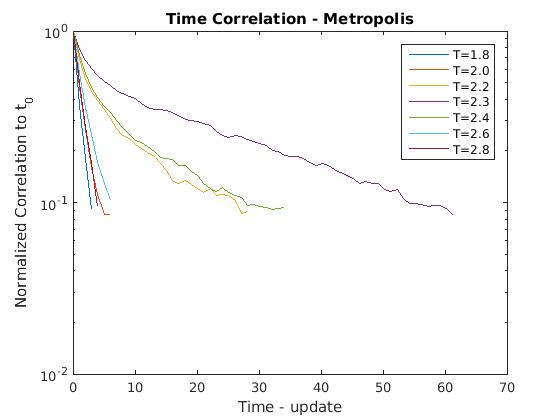
\includegraphics[width=1\textwidth]{../../plots/timeCorrMetro}
	\caption{Here we can see the logarithmic plot of the correlation between energies using the metropolis method for up to 70 time steps. One timestep corresponds to one call of the update function. The plot is made for a 64x64 system and has ben running at different temperature. we can clearly see extra correlation around the critical temperature ~2.3}
	\label{fig:timeCorrMetro}
\end{figure}

\begin{figure}[H]
	\centering
	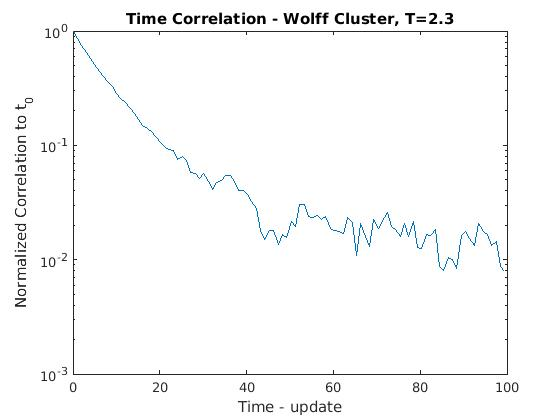
\includegraphics[width=1\textwidth]{../../plots/timeCorrWolf}
	\caption{Here we can again see the magnitude of correlation in the energy at different time steps, but using wolf at T=2.3. As we can see it is considerably larger.}
	\label{fig:timeCorrWolf}
\end{figure}


\begin{table}[h]
  \caption{Correlation time at different temperatures}
  \begin{tabular}{| c | c c c c c c c|}
  \hline
	Temperature (K) & 1.800000 & 2.000000 & 2.200000 & 2.300000 & 2.400000 & 2.600000 & 2.800000\\
	\hline
	Correlation Time (tu) & 3.449311 & 7.675287 & 52.577967 & 115.338197 & 65.874539 & 7.505328 & 4.709923\\
	\hline
  \end{tabular}
  \label{table:timeCorr}
\end{table}

\section{Visualisation of the simulation process}
Using the g2 library i have written a visualisation routine that can with the proper compiler flag be activated at compile time. snapshot if it is depicted in figure \ref{fig:metroVisualization} and \ref{fig:clusterVisualization}. Its a clear difference between the methods while running it, but it does not translate well into pictures. 

\begin{figure}[H]
	\centering
	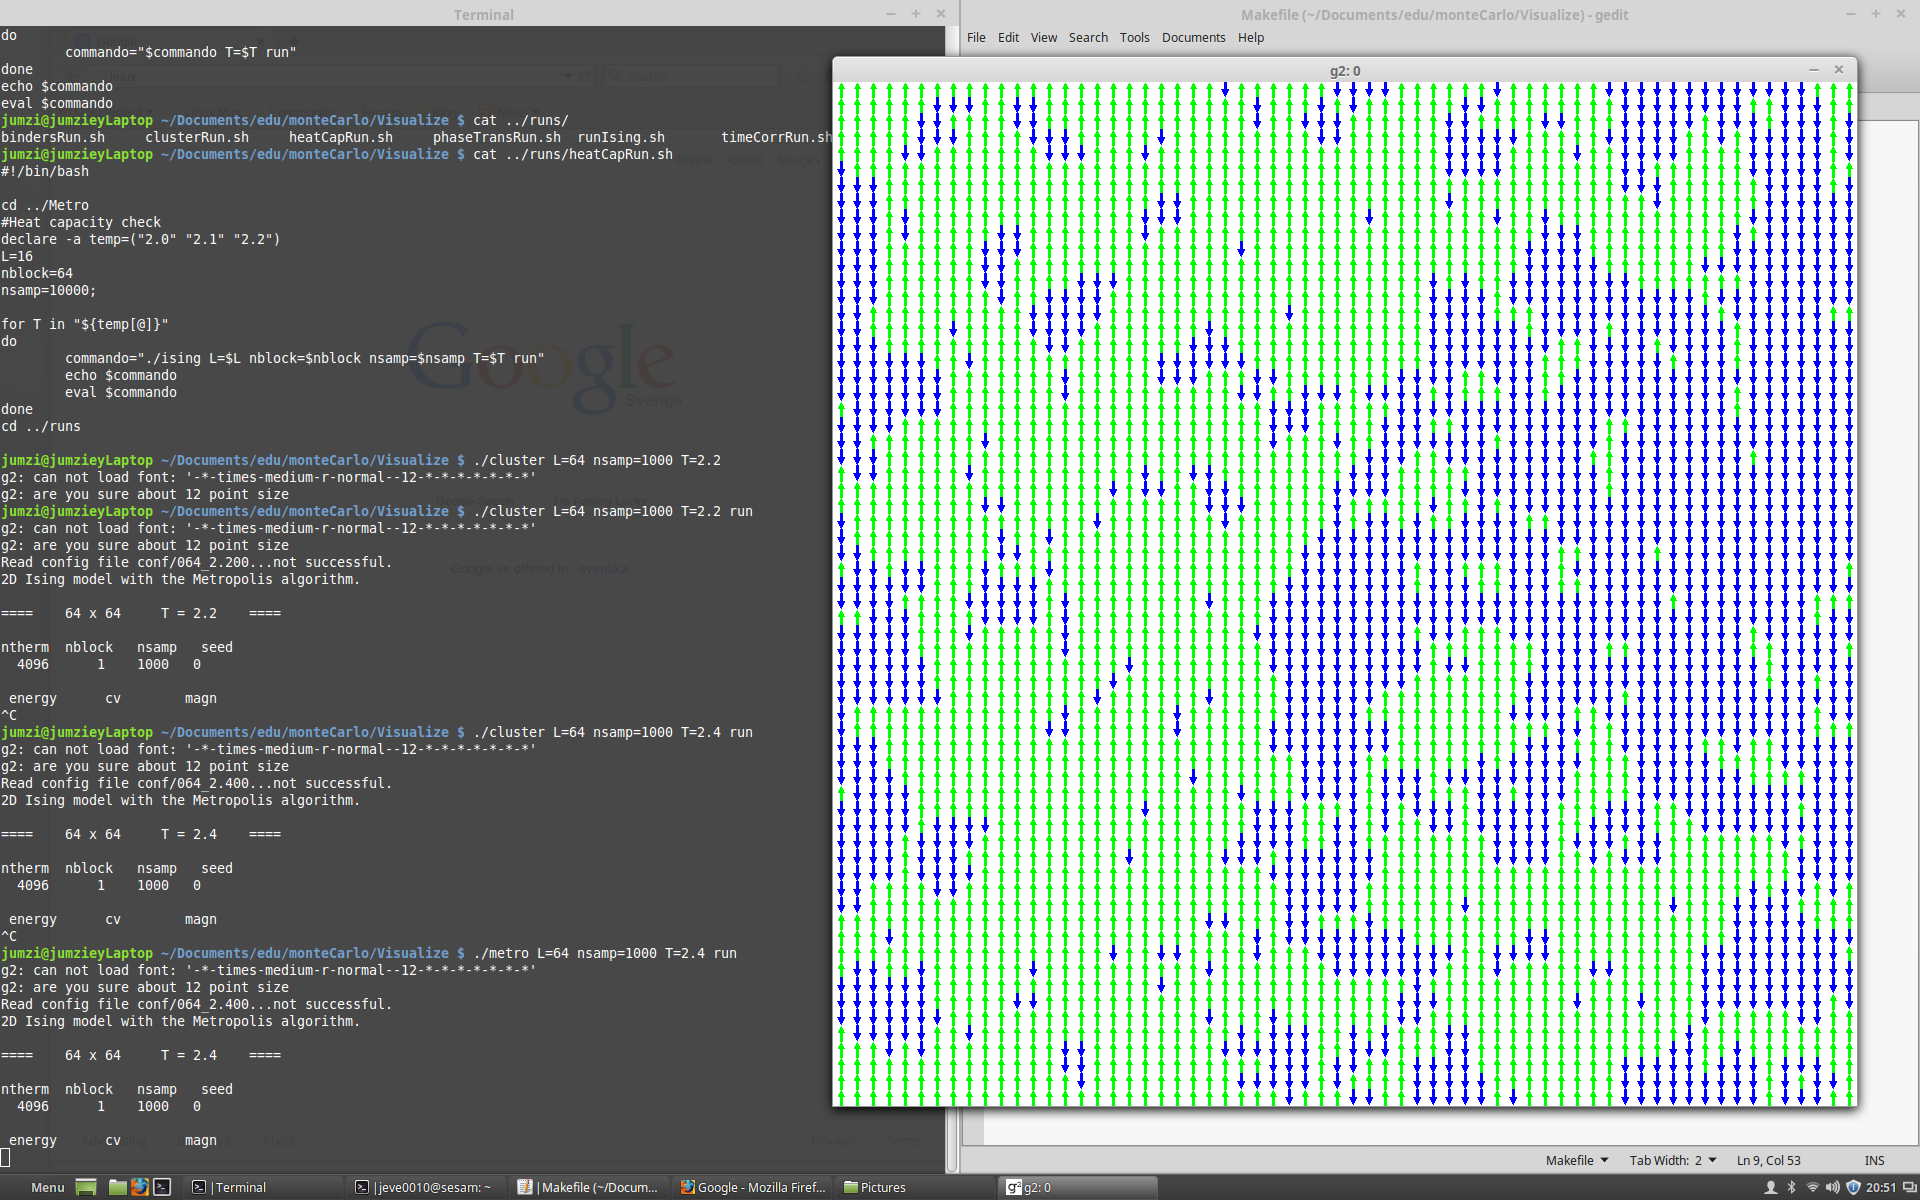
\includegraphics[width=1\textwidth]{../../plots/metroVisualization}
	\caption{Here we can see a snapshot of the visualization process running the simulation software with the metro method}
	\label{fig:metroVisualization}
\end{figure}

\begin{figure}[H]
	\centering
	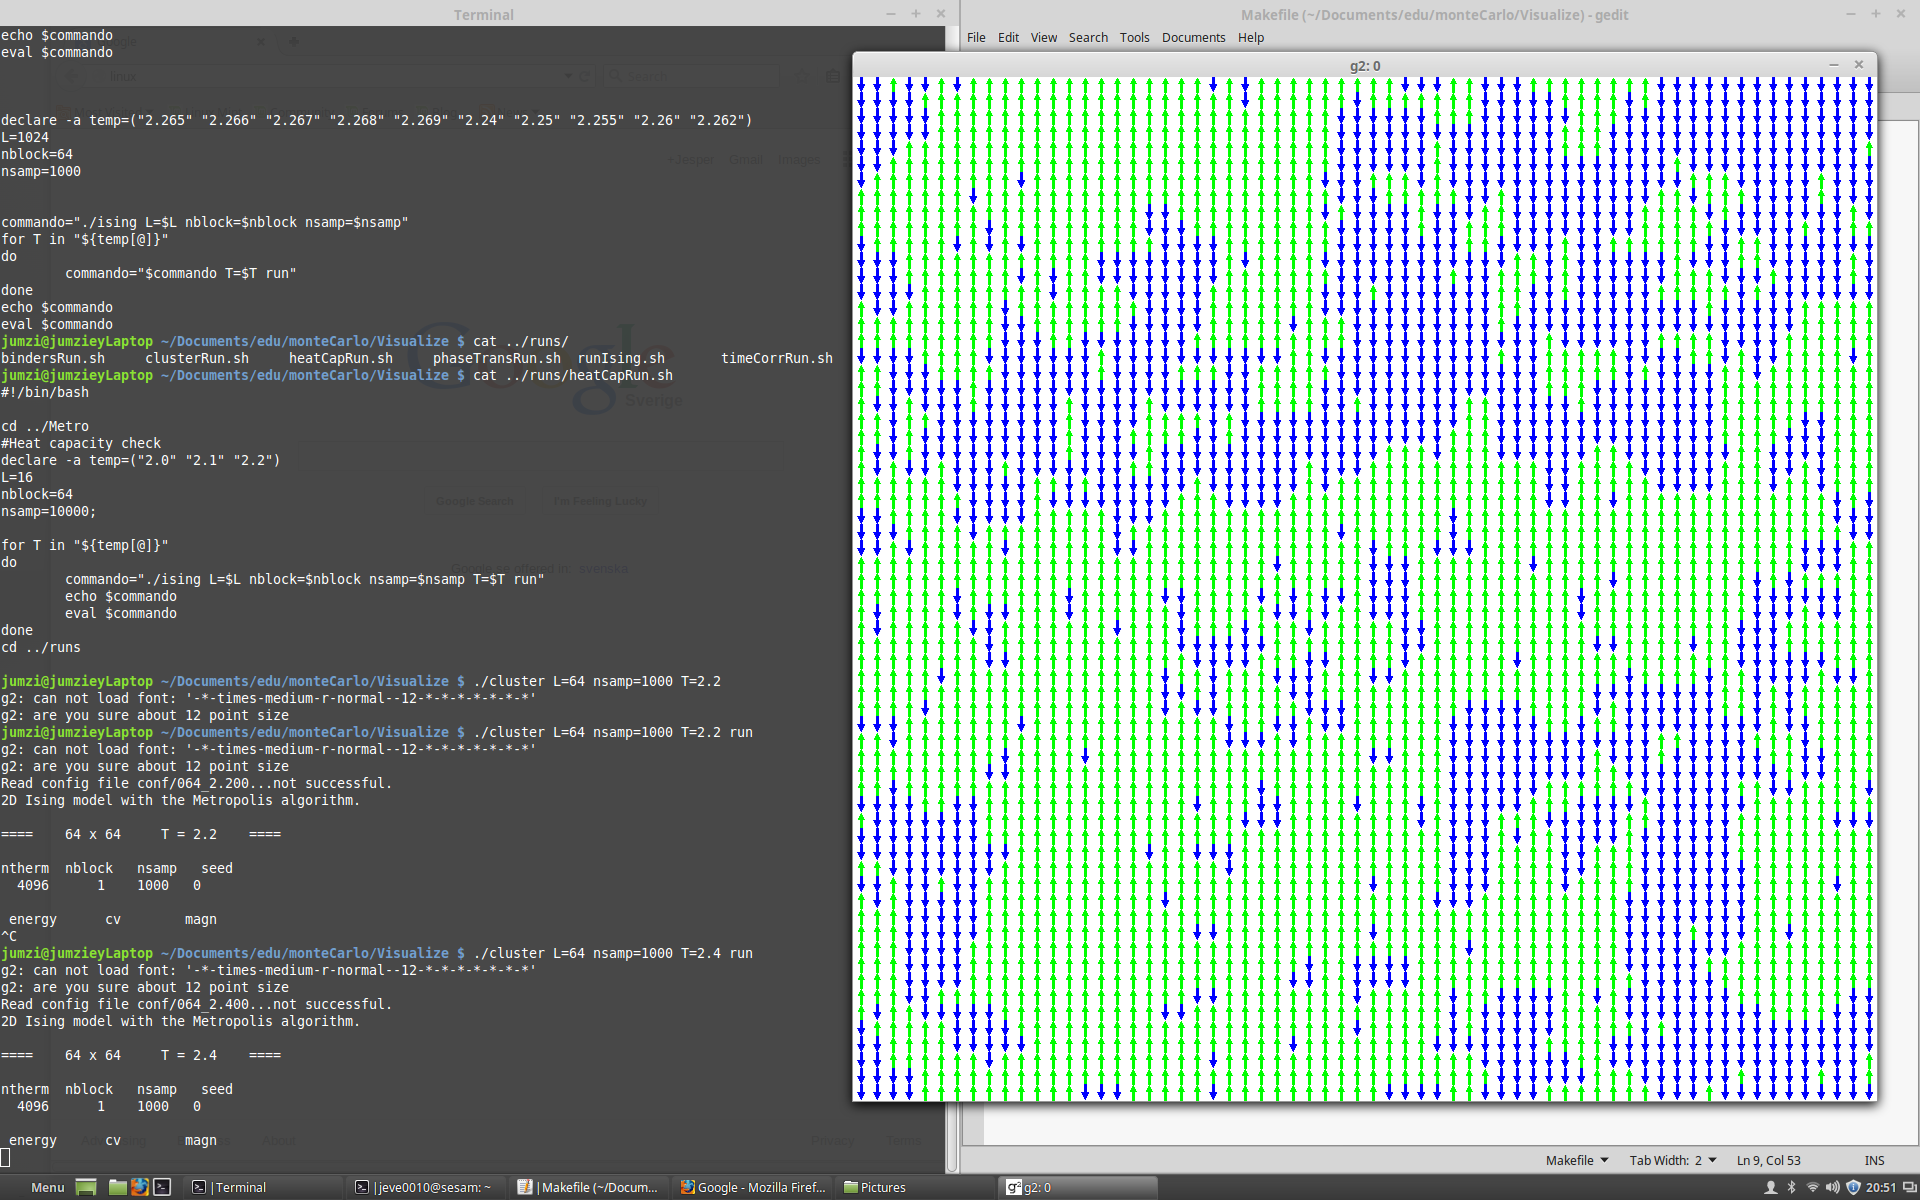
\includegraphics[width=1\textwidth]{../../plots/clusterVisualization}
	\caption{Here we can see a snapshot of the visualization process running with the simulation software with the cluster method}
	\label{fig:clusterVisualization}
\end{figure}





\end{document}
